% Q20: cuboid with the marked midpoints and required segments.
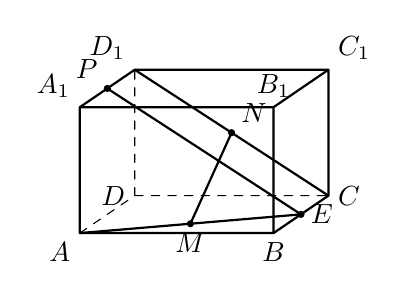
\begin{tikzpicture}[line cap=round,line join=round,x=0.82cm,y=0.82cm]
  \coordinate (A) at (0,0);
  \coordinate (B) at (3,0);
  \coordinate (C) at (3.85,0.58);
  \coordinate (D) at (0.85,0.58);
  \coordinate (Aone) at (0,1.95);
  \coordinate (Bone) at (3,1.95);
  \coordinate (Cone) at (3.85,2.53);
  \coordinate (Done) at (0.85,2.53);
  \coordinate (P) at (0.425,2.24);
  \coordinate (E) at (3.425,0.29);
  \coordinate (M) at (1.7125,0.145);
  \coordinate (N) at (2.35,1.555);

  % Rear edges are dashed; the front and right faces remain visible.
  \draw[dashed] (A)--(D) (D)--(C) (D)--(Done);
  \draw[thick] (A)--(B)--(C) (B)--(Bone)--(Cone)--(C)
               (A)--(Aone) (Aone)--(Bone) (Aone)--(Done)--(Cone) (A)--(B);
  \draw[thick] (A)--(E) (C)--(Done) (M)--(N) (P)--(E);
  \fill (P) circle (1.3pt) (E) circle (1.3pt) (M) circle (1.3pt) (N) circle (1.3pt);
  \node[below left] at (A) {$A$};
  \node[below] at (B) {$B$};
  \node[right] at (C) {$C$};
  \node[left] at (D) {$D$};
  \node[above left] at (Aone) {$A_1$};
  \node[above] at (Bone) {$B_1$};
  \node[above right] at (Cone) {$C_1$};
  \node[above left] at (Done) {$D_1$};
  \node[above left] at (P) {$P$};
  \node[right] at (E) {$E$};
  \node[below] at (M) {$M$};
  \node[above right] at (N) {$N$};
\end{tikzpicture}
